\graphicspath{{chapters/notes/09/images/}}
\chapter{Extracellular vesicles}

\section{Introduction}

    \subsection{Definition}
    Extracellular vesicles are membrane-enclosed nanoscale particles released from essentially all prokaryotic and eukaryotic cells that carry proteins, lipids, RNA and DNA.

    \subsection{Compartments of extracellular vesicles}
    Different compartments of extracellular vesicles can be identified.
    Figure \ref{fig:ev1} represents all the main components of a vesicle.

    \begin{figure}[H]
        \centering
        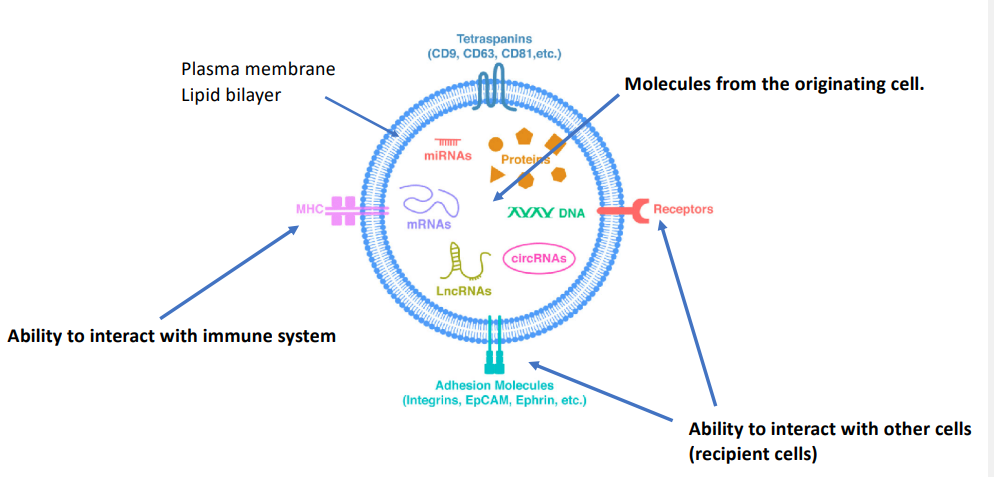
\includegraphics[width=0.5\textwidth]{ev1.png}
        \caption{Sketch representing the main components of an EV.}
        \label{fig:ev1}
    \end{figure}

        \subsubsection{Outside layer}
        The outside layer of extracellular vesicles is made of the lipidic membrane of the cells from which the vesicles were originated.

        \subsubsection{Content}
        The content of extracellular vesicles can vary.
        The can contain:

        \begin{multicols}{3}
            \begin{itemize}
                \item RNAs of different length.
                \item DNA.
                \item Proteins.
            \end{itemize}
        \end{multicols}

        This molecules are derived from the cell that originated the vesicle.

        \subsubsection{Membrane proteins}
        On the membrane of extracellular vesicles there are proteins that are able to to interact with:

        \begin{multicols}{4}
            \begin{itemize}
                \item The immune system.
                \item Receptors.
                \item Adhesion molecules.
                \item Tetraspanins.
            \end{itemize}
        \end{multicols}

        Tetraspanins are proteins that span the membrane four times and act as markers or recognition proteins of the vesicle.

    \subsection{Characterization of extracellular vesicles}
    Extracellular vesicles are very different from each other.
    Especially in older studies, each research group used to study extracellular vesicles from a certain site and gave them a specific name, for example:

    \begin{multicols}{2}
        \begin{itemize}
            \item EVs from the prostate were called \textit{prostatosomes}.
            \item EVs from a tumor sample were called \textit{oncosomes}.
        \end{itemize}
    \end{multicols}

    A consortium was created to order the nomenclature and to determine which are the parameters to characterize and study extracellular vesicles.

        \subsubsection{Size}
        Extracellular vesicles can be characterized by their size:

        \begin{multicols}{2}
            \begin{itemize}
                \item $100$-$1000nm$: microvesicles.
                \item $50$-$150nm$: exosomes.
                \item $100$-$5000nm$: apoptotic extracellular vesicles and apoptotic bodies.
                \item $30$-$50nm$ and no lipid bilayer: exomeres.
            \end{itemize}
        \end{multicols}

        The categories overlap and there is no clear cut.

        \subsubsection{Origin}
        Extracellular vesicles can be further categorized according to their origin:

        \begin{multicols}{2}
            \begin{itemize}
                \item Exosomes originate from the endocytic pathway.
                \item Microvesicles and apoptotic bodies originate from the plasma membrane.
            \end{itemize}
        \end{multicols}

        In particular microvesicles originate directly from the membrane of the cell, while the exosomes come from the multivesicular body, which contains the intraluminal vesicles, as shown in panel a) of figure \ref{fig:origin}.
        Apoptotic bodies instead are the result of cell death.
        In the experiment performed in panel b) of figure \ref{fig:origin}, the researchers induced apoptosis using different methods and the vesicles had different sizes.

        \begin{figure}
            \begin{tabular}{cc}
                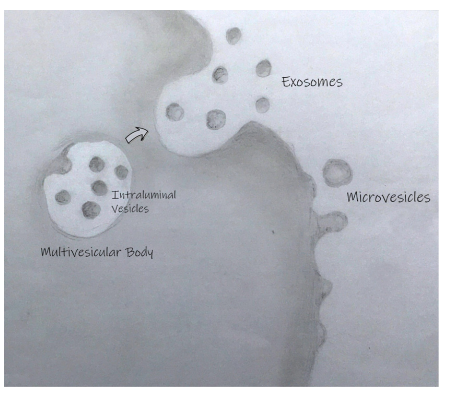
\includegraphics[width=65mm]{origin1} &   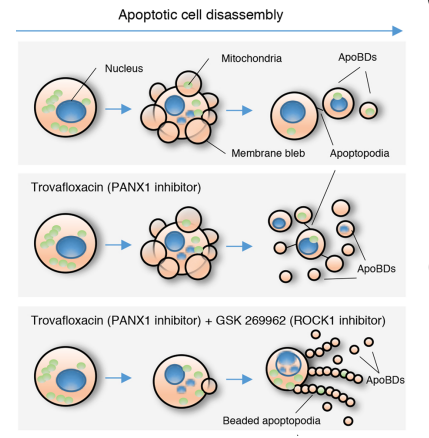
\includegraphics[width=65mm]{origin2} \\
                (a) Origin of exosomes and microvesicles & (b) Origin of apoptotic body \\[6pt]
            \end{tabular}
                \caption{Origin of EVs}
            \label{fig:origin}
        \end{figure}

            \paragraph{Process of origin of exosomes}
            Exosomes are the most interesting extracellular vesicles and originate from a multi-step process:

            \begin{multicols}{2}
                \begin{enumerate}
                    \item Endocytosis: the cell either capture everything in the ECM, or the substrate is selected by receptors.
                    \item Formation of early and late endosomes: lysosomes are organelles which go through a process of maturation, in the late endosomes enzymes complete the packaging of the substrate.
                    \item Formation of multivesicular bodies: multivesicular bodies contain intralumenal vesicles, the precursors of the exosomes.
                \end{enumerate}
            \end{multicols}

        \subsubsection{Content}

            \paragraph{Exosomes and microvesicles}
            Exosomes and microvesicles mainly carry:

            \begin{multicols}{2}
                \begin{itemize}
                    \item Proteins.
                    \item Nucleic acids:

                        \begin{itemize}
                            \item mRNA.
                            \item miRNA.
                            \item other non-coding RNAs.
                        \end{itemize}
                \end{itemize}
            \end{multicols}

            Vesicles are really smalls and cannot contain big fragments of DNA.
            Further studies however proved the presence of longer, protein coding transcripts.
            A lot of RNA transcripts have important regulatory functions like miRNA or circRNA.

            \paragraph{Apoptotic bodies}
            Apoptotic bodies instead are the entire representation of the cell's cytoplasm.
            The contain an equal representation of the cell content.

            \paragraph{Exosomes}
            Exosomes select their cargo through an active process in which:

            \begin{multicols}{2}
                \begin{enumerate}
                    \item Abundant RNA is selected.
                    \item Fragmentation of the RNA occurs.
                    \item RNA is selected through:

                        \begin{itemize}
                            \item Specific sequence motifs.
                            \item Unique secondary structures.
                            \item RNA modification like mRNA uridylation.
                        \end{itemize}

                \end{enumerate}
            \end{multicols}

    \subsection{Functions of extracellular vesicles}
    Each extracellular vesicle carries information about its cell of origin and its putative function.
    Each extracellular vesicle can have a different function, based on the presence on other recipient cells.

        \subsubsection{Functions of extracellular vesicles in cancer}
        In cancer, EVs have important functions.
        In prostate cancer it has been shown that exosomes are able to modulate the immune system, by changing the preferential maturation of the cells of the immune systems.
        They aid in the proliferation of endothelial cells, in stromal fibroblast differentiation, creating population that are pro/anti tumorigenic.
        They remodel the ECM, which is extremely important for metastasis, as EVs provide for a way for cells to bind to a different substrate and create metastatic sites (especially for bone cancer).
        An example of how exosomes can boost metastasis is reported in figure \ref{fig:ev-prostate}, in which prostate cancer extracellular vesicles mediate intercellular communication with bone marrow cells and promote metastasis in a cholesterol-dependent manner.
        In this process exosomes from prostate cancer travel in the body, arrive to the bone and boost metastasis.

        \begin{figure}[H]
            \centering
            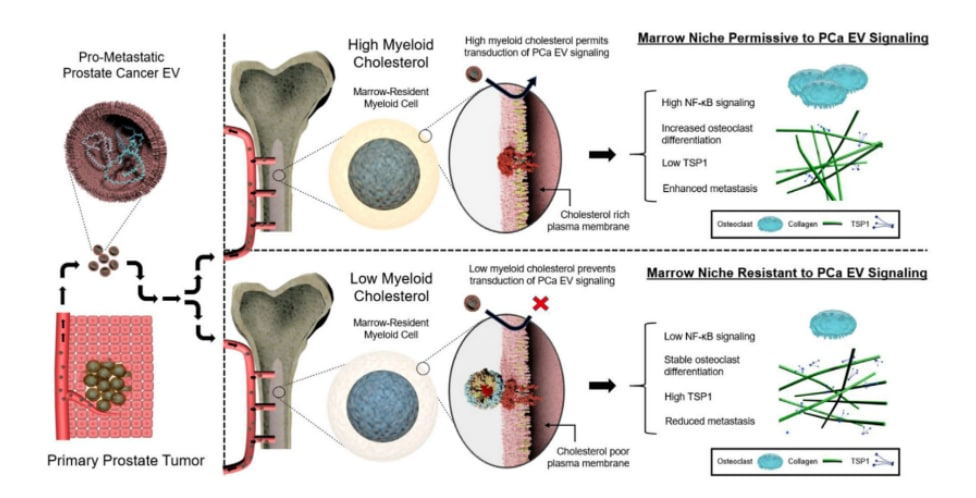
\includegraphics[width=0.5\textwidth]{cancer1.png}
            \caption{Exosomes-mediated metastasis in prostate cancer.}
            \label{fig:ev-prostate}
        \end{figure}

\section{Tumour studies through extracellular vesicles analysis}

    \subsection{Introduction}
    Liquid biopsies can ve used as a novel tool for cancer detection and monitoring.
    By just drawing some blood in a serial matter a lot of extracellular vesicles coming from all body's tissues, including cancer cells, can be retrieved.
    This is of importance because in the same tumour there could be different populations, each harbouring different mutations and having different proliferation rates.
    This cause them to respond in different ways to therapies.
    Liquid biopsies allow to analyse data coming from:

    \begin{multicols}{2}
        \begin{itemize}
            \item Tumour.
            \item Cell free DNA.
            \item Extracellular vescicles.
            \item Ribolipoproteins.
        \end{itemize}
    \end{multicols}

    Analysis of liquid biopsies can be considered with a multi-analyte approach using different molecular cues, coming for example, from DNA and RNA, to detect tumour related signal.

    \subsection{Breast cancer - an example}

    \begin{figure}[H]
        \centering
        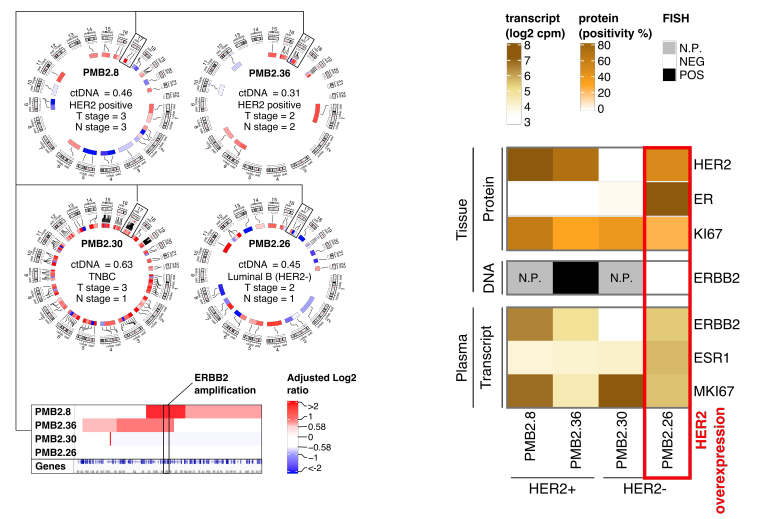
\includegraphics[width=0.5\textwidth]{cancer2.png}
        \caption{4 Breast cancer patients. On the left:  Whole Exome Sequencing of cfDNA from plasma.}
        \label{fig:cancer2}
    \end{figure}

    Breast cancer usually stratifies in different subtype and one of the main molecular feature to distinguish them is the presence of hormone receptors, in particular the one expressed by HER2.
    The experiment depicted in figure \ref{fig:cancer2} collected data from two patients that were HER2 positive and two patients HER2 negative.
    The two positive patients were confirmed by high protein level, but one of the negative patients has a signal for the protein, but no amplification, as the data was collected through FISH.
    The clinicians classified this patient as ambiguous.
    Integrating the data from RNA coming from extracellular vesicles the HER2 positive patient expressed high level of ERBB2, concordant with the previous results, but this data was aslo found for the ambiguous HER2 negative.
    This is concordant with he immuno istochemistry but not by FISH.
    This is because the regulation of HER2 is not only regulated by the amplification, but also by over-expression.
    From this experiment is clear that performing only geneic analysis some information are missed, because with EVs we were able to identify over-expression even in absence of amplification.

    \subsection{Tracking tumour signal in serial samples}
    To track tumour signal evolution a serial approach is taken.
    The signal of different biomarkers is tracked in time.
    This allow to track the response to a drug treatment.
    In this process sequence data from digital PCR of the sample from the blood is performed and the biomarkers are followed in time to discover how well the patient is responding to the treatment.

    \subsection{Extracellular vesicles isolation methods}
    In literature different ways to isolate EVs are reported:

    \begin{multicols}{2}
        \begin{itemize}
            \item Nickel-base isolation (NBI): exploits the charge of the EVs (negative) using metallic beads.
            \item Size exclusion chromatography (SEC): filter the sample based on the size of the molecule or of the extracellular vesicle.
            \item Ultracentrifugation (UCFG): heaviest molecules are compressed in a pallet, which is discarded, and only the surnatant composed of EVs is retained.
        \end{itemize}
    \end{multicols}

    Usually these three methods are used together because they are not perfect: the extracellular vesicles are heterogeneous and each method is able to isolate different subpopulation.
    This is particularly important in liquid biopsies: collecting only some subpopulation would introduce batch effects in the down-stream analysis.

    \subsection{Challenges in studying tumour evolution through extracellular vesicles}
    Some difficulties do consider when studying tumour evolution through extracellular vesicles are:

    \begin{multicols}{2}
        \begin{itemize}
            \item Evidence of high variability of EVs populations in terms of EVs isolation method.
            \item No standard de facto for the analysis of the EVs transcriptome.
            \item Dealing with plasma samples, multiple populations of EVs are present, some of which are relevant to cancer, while other are not.
            \item The RNA signal deriving from multiple populations is difficult to interpret.
        \end{itemize}
    \end{multicols}

    \subsection{Deconvolution}
    Deconvolution is the process through which, from mixed signal after EVs isolation and RNA sequencing, the different population of vesicles and molecules can be characterized and differentiated.

        \subsubsection{Supervised deconvolution}
        Supervised deconvolution is the standard to perform deconvolution.
        The process is shown in \ref{fig:sup}.
        This process has several limitations, mainly due to the fact that it exploits known signature matrices, making it impossible to detect new extracellular vesicles species.

        \begin{figure}[H]
            \centering
            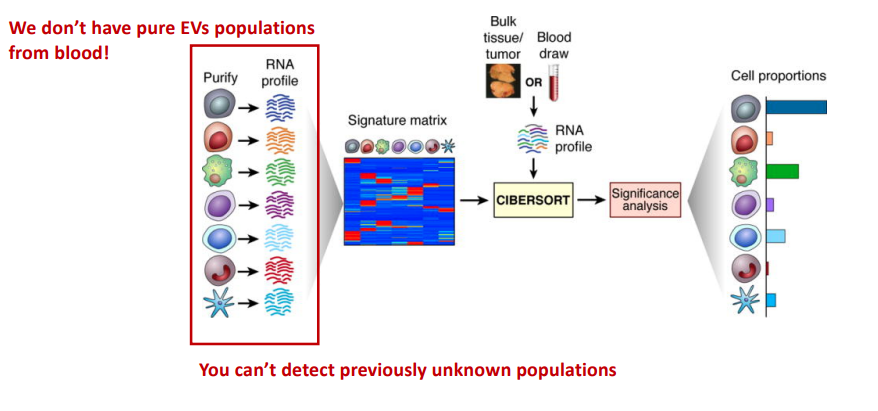
\includegraphics[width=0.7\textwidth]{supervised_devo.png}
            \caption{Supervised deconvolution.}
            \label{fig:sup}
        \end{figure}

        \subsubsection{Unsupervised deconvolution}
        Another possible approach in current development is to implement an unsupervised approach, as the one depicted in figure \ref{fig:unsup}.

        \begin{figure}[H]
            \centering
            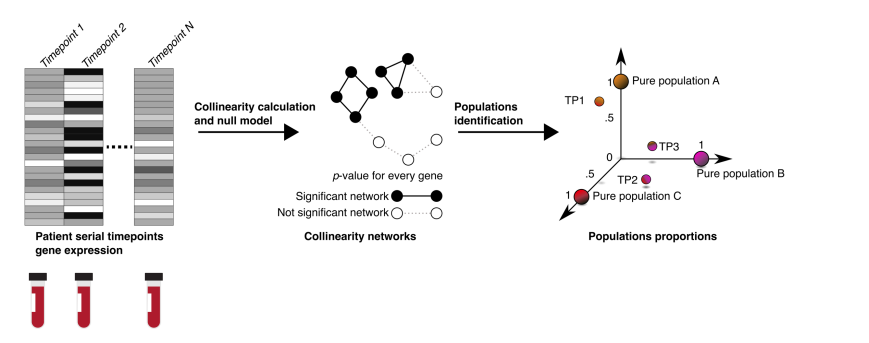
\includegraphics[width=0.7\textwidth]{unsupervised_deco.png}
            \caption{Unsupervised deconvolution.}
            \label{fig:unsup}
        \end{figure}

    \subsection{Conclusion}
    In conclusion it can be said that:

    \begin{multicols}{2}
        \begin{itemize}
            \item Extracellular vesicles can be isolated and analysed from biofluids.
            \item Extracellular vesicles are involved in tumour related processes.
            \item Extracellular vesicles carry information about their cell of origin and function.
            \item Extracellular vesicles populations in blood are heterogeneous.
                Making their analysis difficult.
            \item Deconvolution approaches are possible but not yet well established.
            \item The analysis of extracellular vesicles together with other molecules in liquid biopsies like cfDNA can be more informative in respect to the analysis of a single analyte alone.
                A multi-analyte approach is convenient and increase the predictive power of the analysis.
        \end{itemize}
    \end{multicols}
